\documentclass[a4paper,11pt,openright,oneside]{report}
\usepackage[utf8]{inputenc}
\usepackage[T1]{fontenc}
\usepackage[portuguese]{babel}
\usepackage{graphicx}
\usepackage[backend=biber, style=ieee]{biblatex}
\usepackage{csquotes}
\usepackage{blindtext}
\usepackage[printonlyused]{acronym}
\usepackage{hyperref}
\usepackage{indentfirst}
\usepackage[titletoc,title]{appendix}
\usepackage{mathtools}
\usepackage{amsmath,amsthm,amsfonts,amssymb}
\usepackage{caption}
\usepackage{subcaption}
\newcommand{\RNum}[1]{\uppercase\expandafter{\romannumeral #1\relax}}

\bibliography{report.bib}

\begin{document}

\begin{titlepage}
\begin{center}

{\vspace*{50mm}\textsc{\Huge\textbf{Bloom-filter + Locality-Sensitive Hashing}\\ \small{Métodos Probabilísticos para Engenharia Informática}}}\\[2cm]
{\textsc{\small\textbf{Universidade de Aveiro}}}\\[0.5cm]
{\small Pedro Martins 76551\\Ricardo Jesus 76613}\\[0.5cm]
{\small	17 de Dezembro de 2015}\\

\begin{figure}[b]
\center
\graphicspath{}

\includegraphics[height=2cm]{ua.pdf}
\end{figure}

\end{center}

\end{titlepage}

\title{\textbf{Bloom-filter + Locality-Sensitive Hashing}\\[1cm]\textsc{\small {Departamento de Electrónica, Telecomunicações e Informática} \\ \large {UNIVERSIDADE DE AVEIRO}}}
\author{Pedro Martins 76551, pbmartins@ua.pt\\Ricardo Jesus 76613, ricardojesus@ua.pt}
\date{17 de Dezembro de 2015}

\maketitle

\pagenumbering{roman}

\begin{abstract}

ABSTRACT

\end{abstract}

\tableofcontents
%\listoftables
\listoffigures

\clearpage
\pagenumbering{arabic}

\chapter{Introdução}
\label{chap.introdução}

Na área da informática, é, por exemplo, muitas vezes necessário saber se algo pertence a um certo conjunto de forma eficiente. A solução mais óbvia seria percorrer todo o conjunto e comparar, um a um, todos os elementos até encontrar aquele de que se andava inicialmente à procura. No entanto, este método é deveras ineficiente, principalmente se se estiver a trabalhar com conjuntos com milhões ou mais elementos. É aqui que surgem estruturas como \textit{Bloom-filters}. 

\textit{Bloom-filters} usam geralmente várias funções de dispersão (ou \textit{hashing}) para determinar a pertença de um dado elemento num conjunto (\textit{set}). São muito utilizados em grandes conjuntos de dados e em diversas aplicações, como corretores ortográficos de computadores, \textit{smartphones}, etc., análise textual, entre outras. Contudo, e sendo uma estrutura probabilística, acarreta um erro associado.

Outra técnica bastante relevante em situações onde é ``impossível'' guardar e trabalhar enormes conjuntos de dados é o de \textit{MinHash}. Muitas vezes a par com este aparece também o método de \textit{Locality-sensitive hashing (LSH)}, com aplicações usuais em \textit{clustering} de informação e procura de vizinhos próximos a um dado elemento (\textit{nearest neighbor search}).

Neste trabalho, foi desenvolvido em MATLAB um \textit{Bloom-filter}, um \textit{MEX file} fazendo de interface para uma função de \textit{hashing} escrita em C++ e ainda um módulo com capacidade de \textit{nearest neighbor search} utilizando \textit{MinHash} para gerar uma representação de diferentes documentos a serem tratados.

\chapter{Bloom-filter}
\label{chap.bloom}

\textit{Bloom-filters} são estruturas de dados probabilísticas que utilizam uma ou várias funções de \textit{hashing} para determinar a pertença de um dado elemento num \textit{set}. Internamente, habitualmente utilizam um vector de \textit{bits}. Neste trabalho utilizou-se um vetor de \textit{bytes} visto que a linguagem em que o módulo foi escrito (MATLAB) não suporta o tipo \textit{bit}. Para se tirar partido do espaço extra que se utilizou, o módulo foi implementado como um \textit{Counting filter}, onde portanto se mantém registo do número de elementos semelhantes que deverão ter sido adicionados ao filtro.

Assumindo funções de \textit{hashing} eficiêntes, mesmo que se opere sobre um conjunto com milhões ou milhares de milhões de elementos, determinar a presença ou não presença nesse conjunto será sempre um processo significativamente mais rápido que caso se iterasse sobre todo o \textit{set}, elemento a elemento, à procura daquele em questão. Este processo depende do número e da qualidade das funções de \textit{hashing} utilizadas, bem como do tamanho do vetor interno..

Como estrutura probabilística que é tem um erro associado, neste caso manifestando-se apenas em falsos positivos, i.e., se um \textit{Bloom-filter} indica que um elemento pertence a um conjunto, então \underline{provavelmente} ele pertence mesmo. Por outro lado, se um \textit{Bloom-filter} indica que um elemento não pertence a um conjunto, então \underline{definitivamente} ele não pertence. Tendo isto em mente, habitualmente os \textit{Bloom-filters} são dimensionados para um erro máximo admissível e para um determinado número de elementos que se tencione adicionar ao filtro.

Este erro depende do número de \textit{buckets} no vector interno e do número de funções de \textit{hashing} a utilizar. Estas funções devem ser descorrelacionadas entre si e em número variável (para cada conjunto de parâmetros para os quais o filtro é dimensionado). Uma solução para o número variável de funções que se deve considerar é, em vez de se utilizarem $k$ funções diferentes, utilizar-se uma família de funções que garanta $k$ funções descorrelacionadas.

Neste trabalho utilizou-se a família de funções de dispersão denominada \textit{FarmHash}, desenvolvida pela Google, em que um dos argumentos, a \textit{seed}, permite especificar cada uma das funções da família. A sua implementação é disponibilizada em C++ pela empresa que a desenvolveu, e portanto de forma a poder ser utilizada ao longo do projeto foi escrito um ficheiro \textit{MEX} que permite a interface entre código MATLAB e a função. Caso seja necessário, o ficheiro pode ser compilado executando (no directório onde os ficheiros \textit{.h} e \textit{.cpp} relativos à função se encontrem) \verb|mex FarmHash.cpp|.

\section{Atributos}
\label{sec.attributes}

Na implementação deste trabalho (ficheiro \textit{BloomFilter.m}) desenvolveu-se uma estrutura baseada num \textit{Counting Bloom-filter} (conta-se o número de vezes que cada elemento é adicionado ao filtro), com 5 atributos:

\begin{description}
\item[k]
Número de funções de \textit{hashing} a utilizar.
\item[byteArray]
Estrutura de dados interna do filtro, vector de \textit{bytes}.
\item[arraySize]
Tamanho do vetor de \textit{bytes}.
\item[amountAdded]
Número total de elementos adicionados ao \textit{array}.
\item[expectedMaxSize]
Tamanho do conjunto que se pretende adicionar do vetor.
\end{description}

\section{Métodos}
\label{sec.methods}

No construtor da classe, são calculados os valores do tamanho do vetor (\texttt{arraySize}) e do número de funções de \textit{hash} necessárias, consoante os valores passados como argumentos do próprio construtor: a probabilidade de falsos positivos, i.e., o erro admissível (\texttt{falsePositiveProbability}) e o tamanho do conjunto que se pretende adicionar ao vetor (\texttt{expectedMaxSize}). 

Assumindo que a probabilidade de falsos positivos é $p$

$$ p =  \left(1 - e^{-\frac{km}{n}}\right)^k $$

e, usando o tamanho do vetor de \textit{bytes} $n$ e o tamanho do conjunto que queremos adicionar ao filtro $m$,

$$ a = \left(1 - \frac{1}{n}\right)^m $$

para determinar o número $k$ ótimo de funções de \textit{hashing} que devem ser utilizadas, deduz-se

$$ \ln p = k * \ln \left(1 - a^k\right) \\
\Leftrightarrow k =  \frac{n * \ln 2}{m}$$

A partir das fórmulas acima encontradas, conclui-se também

$$ n = \frac{m * \ln \left(\frac{1}{p}\right)}{\left(\ln 2\right) ^ 2} $$

Para além do construtor, existem também métodos para adicionar e verificar a existência de elementos no filtro, entre outros:

\begin{description}
\item[add]
Adiciona um elemento ao filtro.
\item[contains]
Verifica se o elemento passado como argumento existe no filtro (poderá haver ocorrência de falsos positivos).
\item[count]
Devolve o número de vezes que um dado elemento foi adicionado ao vetor (apenas uma estimativa).
\item[Setters]
Coleção de funções utilizadas para modificar os atributos do \textit{Bloom-filter}, caso o campo \texttt{debug} (argumento passado ao construtor) esteja com o valor 1.
\end{description}

Existem ainda outros métodos que não foram aqui descriminados visto ou serem privados (e portanto não relevantes à interface do módulo) ou não terem sido testados adequadamente por não terem sido necessários ao longo do trabalho.

\section{Testes}
\label{sec.bloomtests}

Para testar este módulo foram desenvolvidos diversos testes, de entre os quais uns para verificar qual seria o número ideal de funções de \textit{hashing} ($k$) a utilizar, outros para verificar o tamanho ideal do vetor de \textit{bytes} ($n$), outros ainda para verificar que a família de funções de dispersão escolhida tinha um desempenho adequado.

No entanto, também foram realizados outros testes relativamente às funções de \textit{hashing} utilizadas pelo \textit{Bloom-filter}.

\subsection{Distribuição de funções de \textit{hashing}}
\label{subsec.hashdist}

Este módulo (\textit{test\_hashFunction\_distribution.m}) tem como principalmente objetivo provar que as funções de \textit{hashing} têm uma distribuição uniforme para diversos valores de $k$ (neste caso, irá variar entre 1 e 10).

Neste teste, foi gerado um conjunto de \textit{strings} aleatórias, usando a função \texttt{generateStrings}, que aceita como argumentos o tamanho do conjunto que devolverá e o tamanho máximo das \textit{strings} que irá gerar (caso o terceiro argumento seja $0$, terão tamanho fixo, caso contrário tamanho aleatório com máximo especificado pelo segundo argumentoo), e gerados diversos valores de \textit{hashing}, consoante os diversos elementos do conjunto e da \texttt{seed} correspondente.

As distribuições para cada valor de $k$ deverão ser o mais uniformes possíveis, e os resultados estão de acordo, tal como evidênciado pelos histogramas da \autoref{fig:hashdist}.

\begin{figure}[ht]	
\center
\fbox{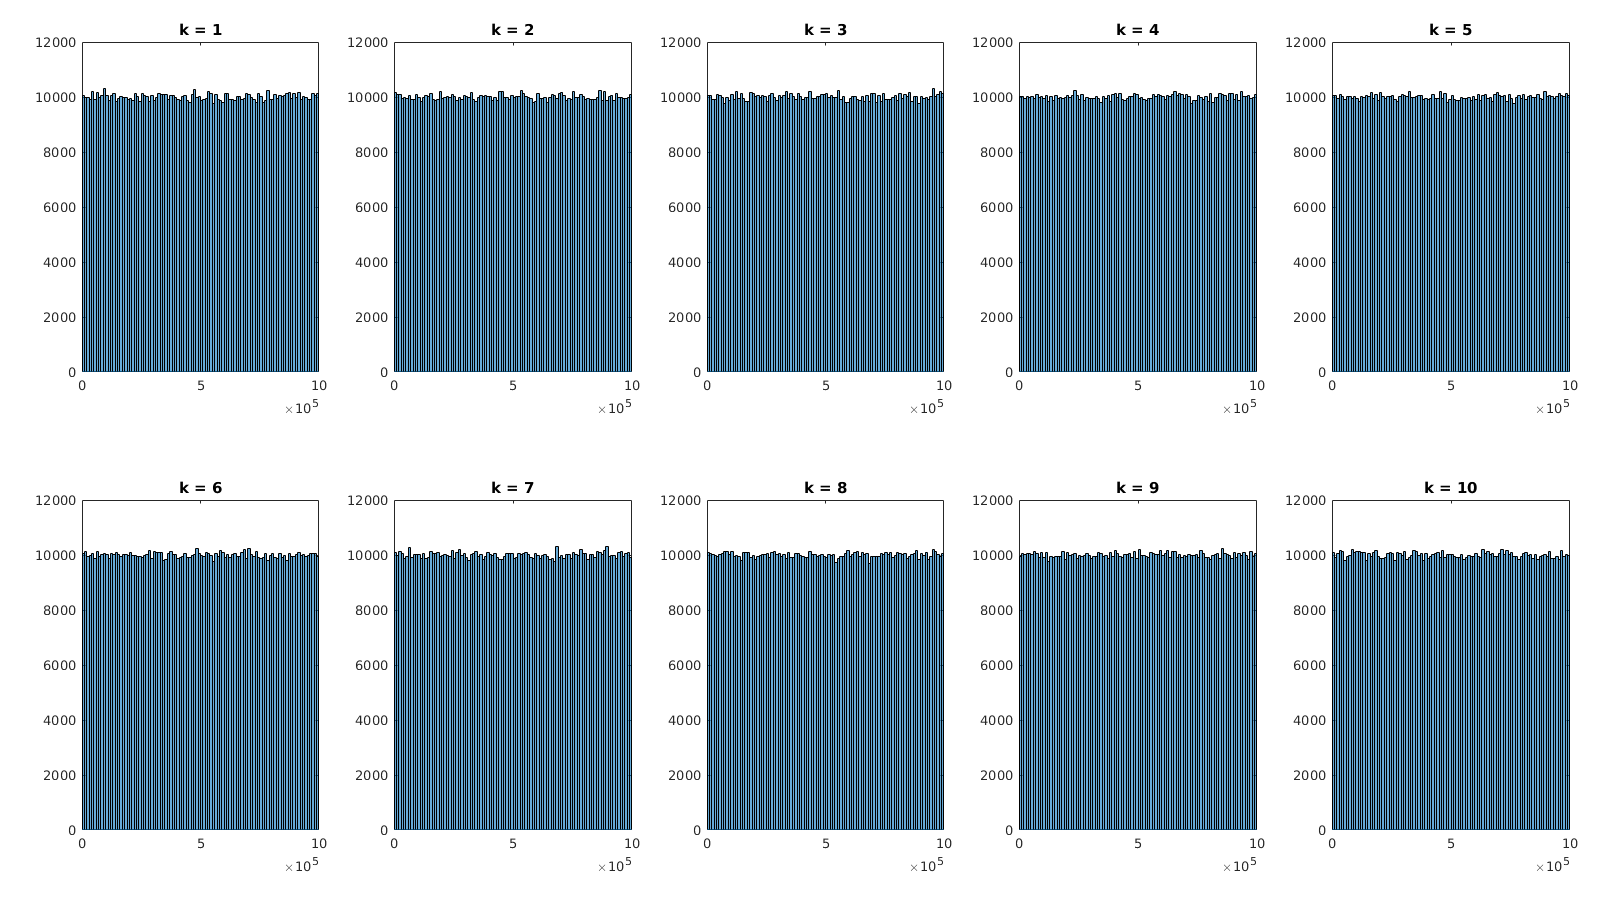
\includegraphics[height=5cm]{img/test_HashFunction_distribution}}
\caption{Resultados das distribuições das \texttt{k} funções de \textit{hashing}}
\label{fig:hashdist}
\end{figure}

\subsection{Correlação das funções de \textit{hashing}}
\label{subsec.hashcorr}

Para que se possam ser utilizar as várias funções de \textit{hashing} eficientemente (neste caso isso significa sem aumento da taxa de falsos positivos), é necessário que estas sejam descorrelacionadas (i.e., que o coeficiente de correlação respetivo seja 0). No entanto, neste trabalho considerar-se-ão valores de coeficiente de correlação inferiores a 0.01 como admissíveis (é muito difícil que estes valores sejam iguais a zero, e portanto aceita-se esta ligeira variação).

Este teste encontra-se no ficheiro \textit{test\_hashFunction\_correlation.m} e, tal como noutros testes, gerar-se-á um \textit{set} de \textit{strings} aleatórias e os respetivos valores de \textit{hashing} para diferentes valores de $k$, a variar entre 1 e 100. No teste, foi criada uma matriz de dimensões $k$ por \texttt{numTests} para guardar as \textit{hashes} para os diferentes pares \textit{k - string}. De seguida, calculam-se os coeficientes de correlação das funções duas a duas utilizando os resultados nas linhas da matriz anterior e a função \texttt{corrcoef} (calcula o coeficiente de correlação entre dois conjuntos, neste caso, duas linhas representativas de dois valores de $k$ distintos).

Por fim, é gerado um gráfico recorrendo à função \texttt{surf} que premite ilustrar os valores de correlação resultantes. Verifica-se que para diferentes valroes de $k$ num par (i.e., comparando $k$s diferentes) os valores se situam geralmente bastante abaixo do erro assumido, havendo alguns picos onde efetivamente o coeficiente de correlação se aproxima deste erro. Conluí-se assim que as funções escolhidas são ``suficientemente'' descorrelacionadas, tal como se pretendia.

\begin{figure}[ht]	
\center
\fbox{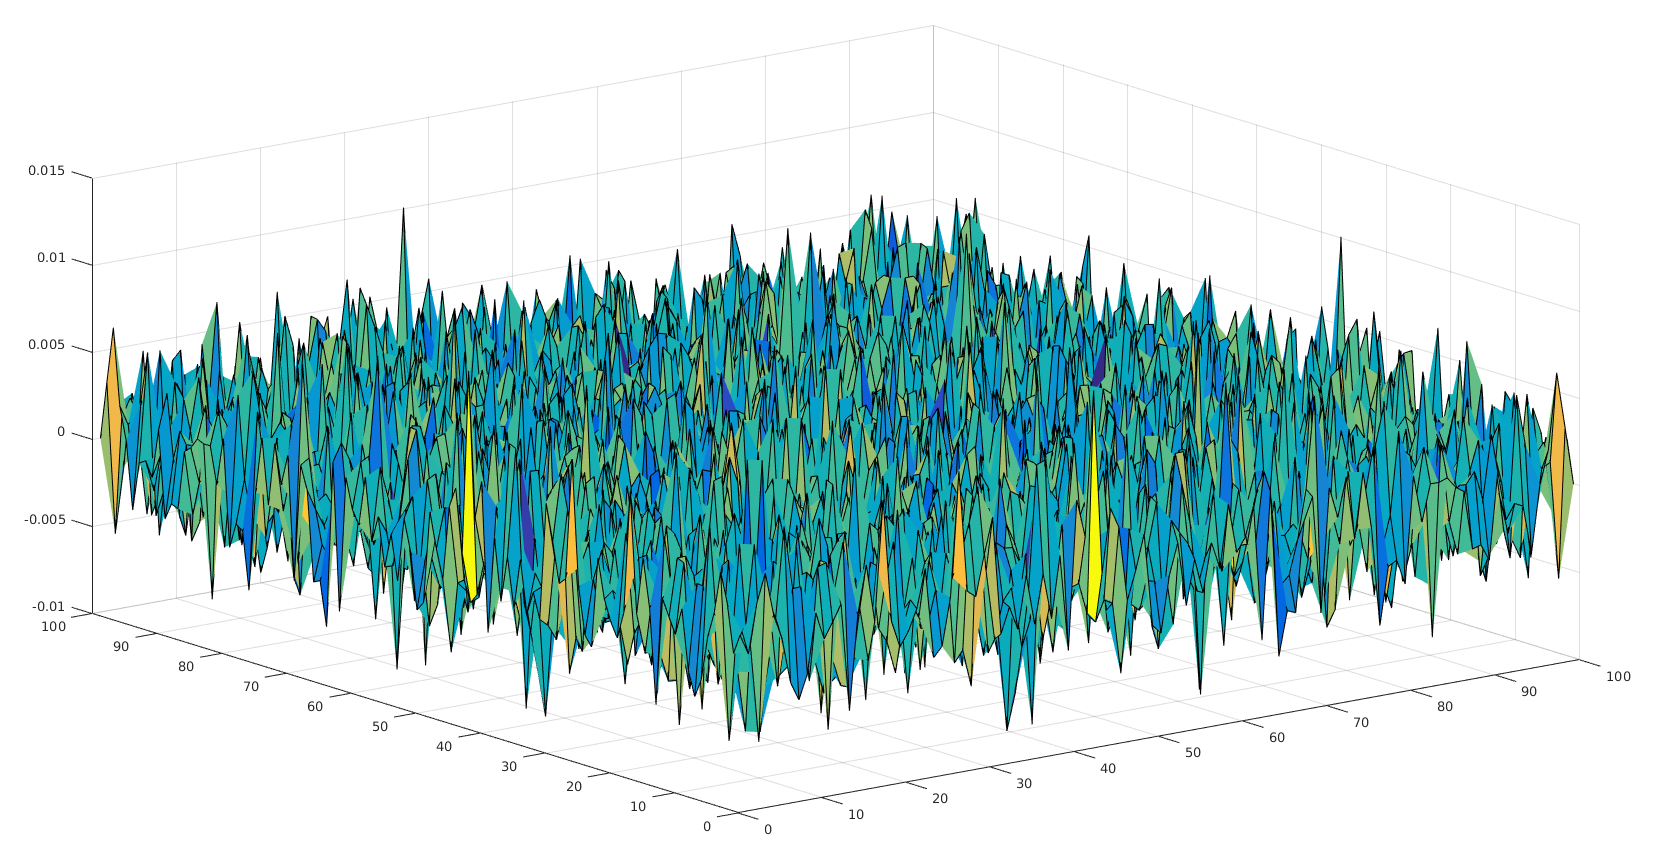
\includegraphics[height=5cm]{img/test_HashFunction_decorrelation}}
\caption{Resultados do teste de correlação de \texttt{k} funções de \textit{hashing}}
\label{fig:hashcorr}
\end{figure}

\subsection{Independência das funções de \textit{hashing}}
\label{subsec.hashindep}

Para além do teste de correlação, foi também efetuado um teste de independência das funções de \textit{hashing} (\textit{test\_hashFunction\_independence.m}), adaptado de uma implementação disponibilizada pelo professor António Teixeira. Visto que independência implica descorrelação, este teste pode ser visto como uma versão mais forte do teste anterior. Analogamente a esse teste, estudou-se a independência das diferentes funções de \textit{hashing} duas a duas.

Primeiramente é criado um \textit{set} de cem mil \textit{strings} aleatórias. De seguida constrói-se uma matriz $n$ (número de \textit{strings} geradas) por $k$ (número de funções de \textit{hashing} da família \textit{FarmHash} que se pretende aplicar, neste trabalho $k = 10$),  onde cada elemento da matriz simboliza o \textit{hash code} dum par (\textit{string}, $k$). Seguidamente, é gerado um vetor de 10 elementos linearmente espaçados (\texttt{x}) entre 0 e \texttt{N} (valor ao qual são limitados os \textit{hash codes}), e, para cada par de colunas, é criada uma matriz (\texttt{pmf}) de dimensão \verb|length(x) - 1| por \verb|length(x) - 1|. Guarda-se então em cada elemento da matriz o número de elementos das colunas de \textit{hash codes} que se situam num mesmo intervalo do vetor \texttt{x} já criado.

Por fim, é calculada a matriz de probabilidade conjunta de duas colunas (\textit{pmf - probability mass function}) dividindo cada elemento da matriz \textit{pmf} anterior pelo número de \textit{strings} que tinham sido criadas. A partir desta, são calculados os vetores de probabilidades individuais correspondentes às linhas e colunas da matriz de probabilidades conjuntas. Finalmente, é calculado o resultado da multiplicação destes dois últimos vetores e verifica-se qual a diferença entre esses valores e os registados na matriz \textit{pmf} (dois acontecimentos $A$ e $B$ são independentes se $P(A\&B) = P(A) * P(B)$).

Como os valores da variação dos resultados são mínimos (como se observa na \autoref{fig:hashindep}, onde todos os valores se encontram na casa dos $10^-4$), podemos considerar que a família de funções é independente dois a dois (pelo menos até ao valor de $k$ considerado), o que permite a concluir que estas funções são descorrelacionadas, tal como verificado anteriormente.

\begin{figure}[ht]	
\center
\fbox{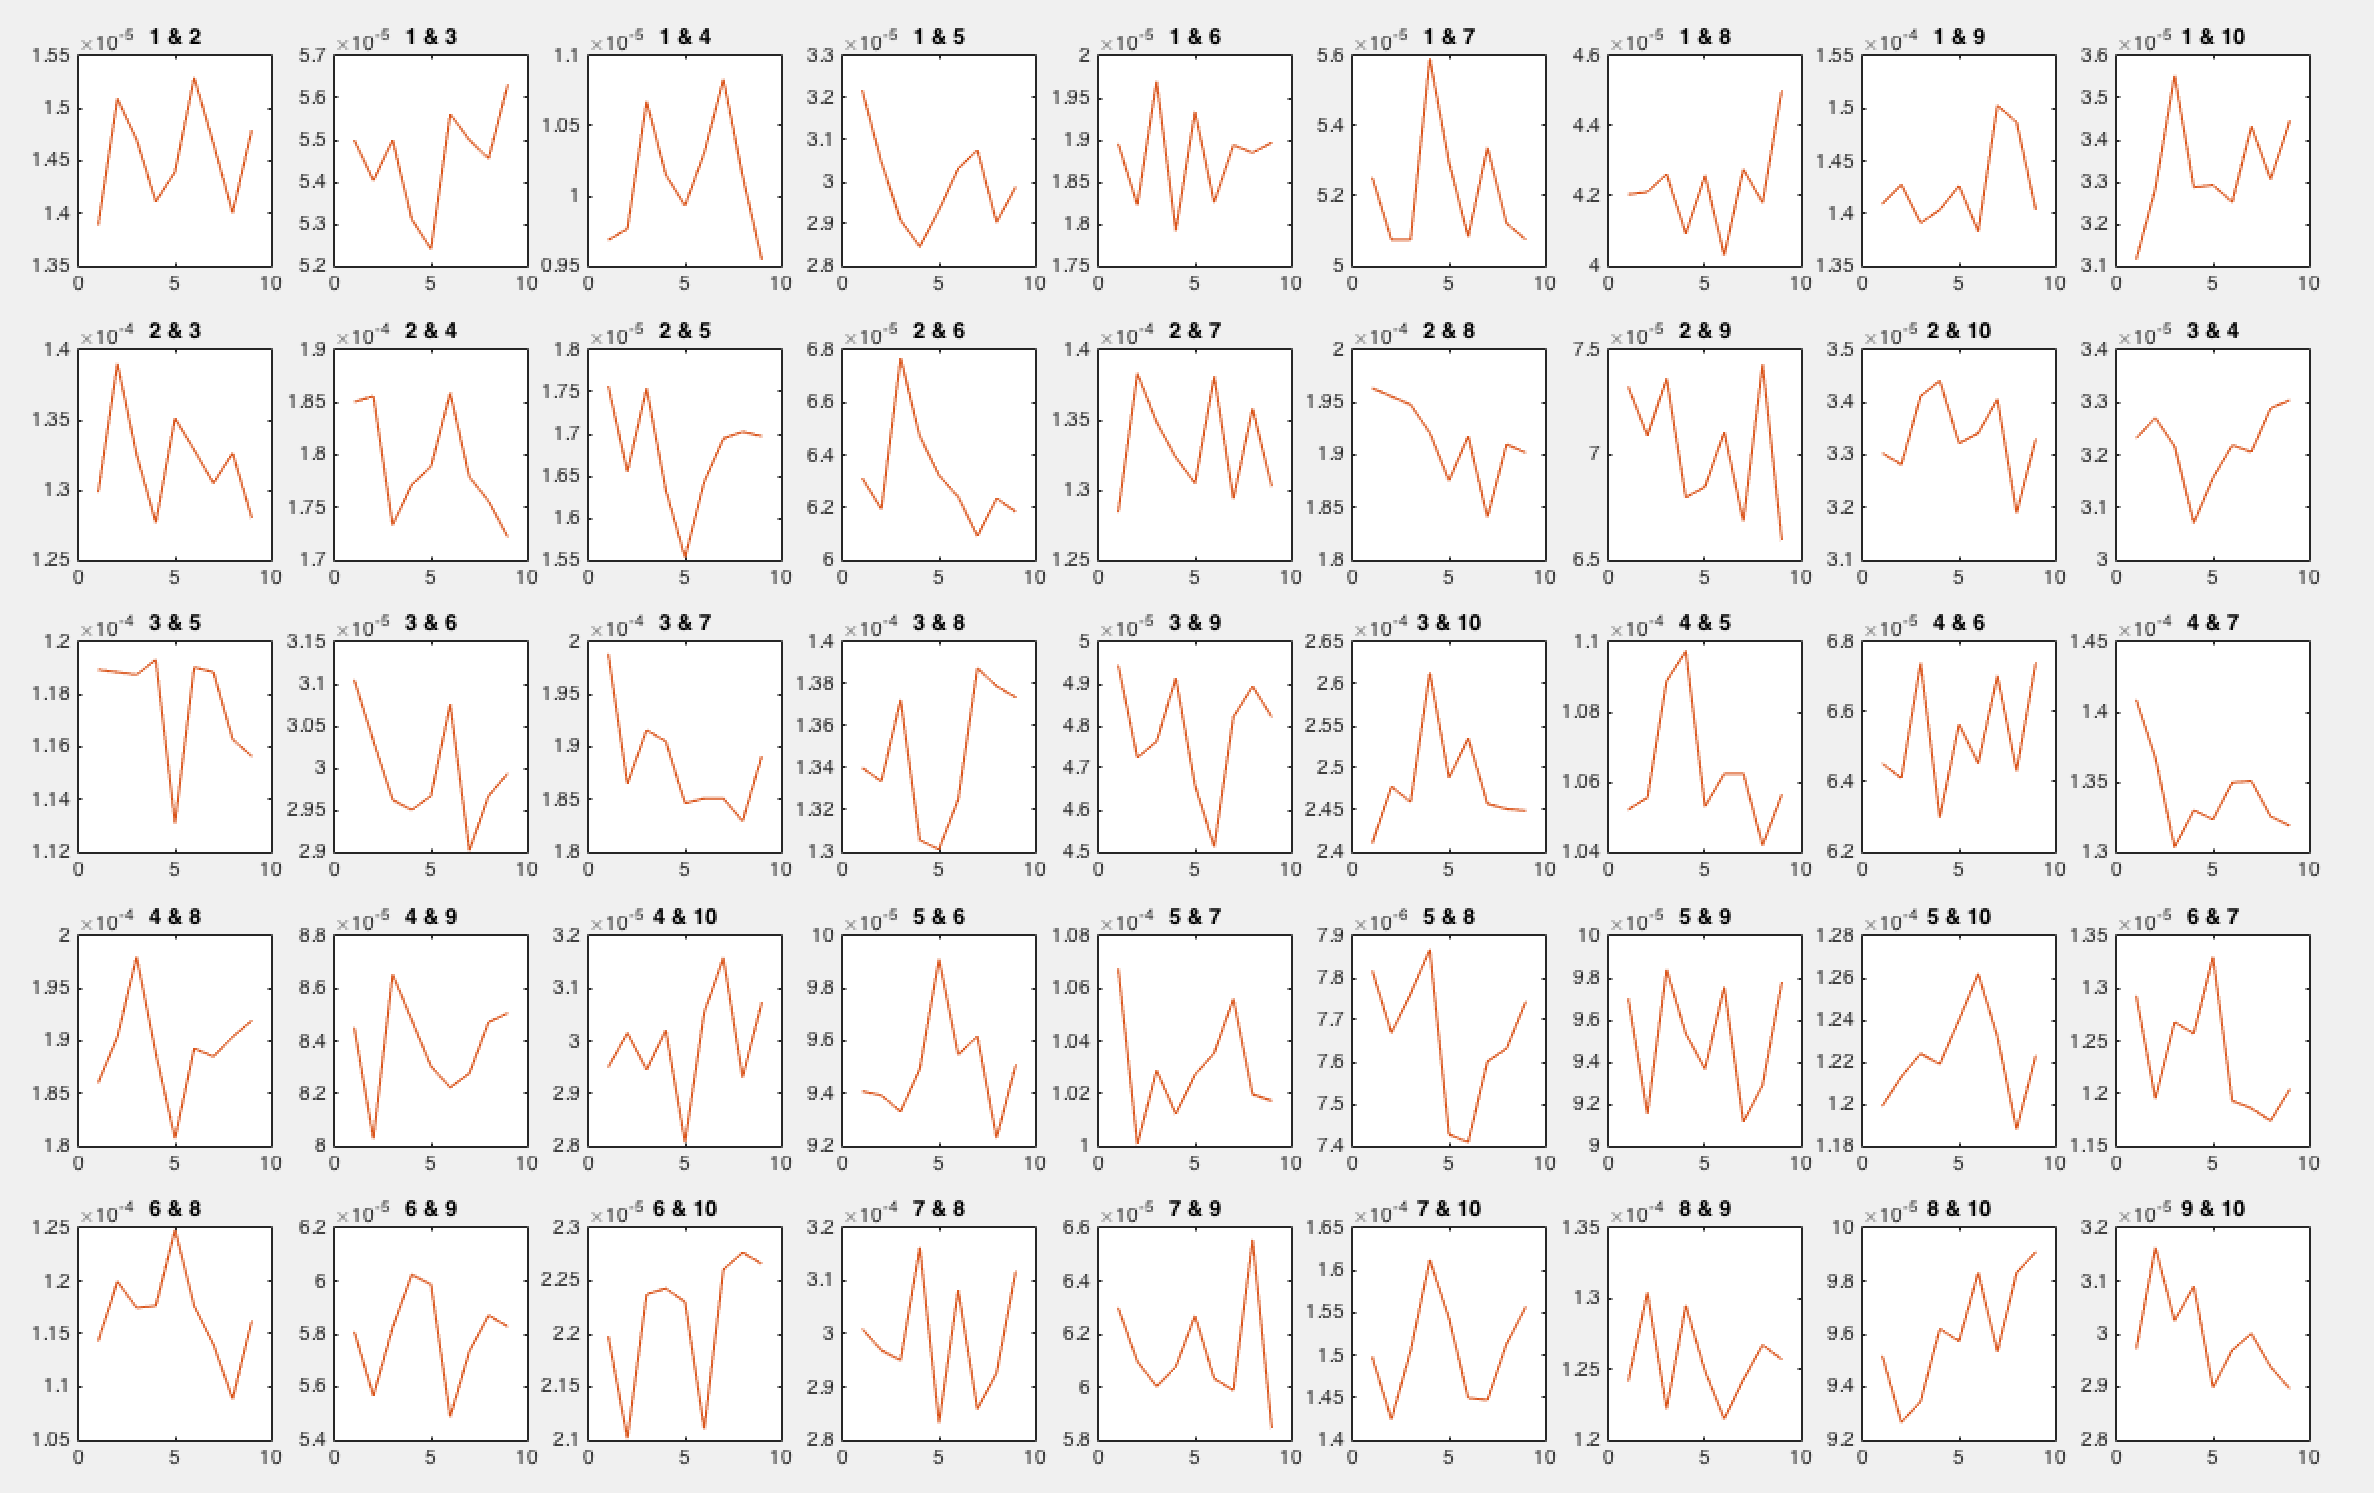
\includegraphics[height=7cm]{img/test_hashFunction_independence}}
\caption{Resultados do teste de independência de \texttt{k} funções de \textit{hashing}}
\label{fig:hashindep}
\end{figure}

\subsection{Número ideal de funções de \textit{hashing}}
\label{subsec.optimalk}

O programa de teste para o valor de $k$ ideal encontra-se com o nome \textit{test\_optimalK.m}.

Começa-se por se criar uma instância da classe de \textit{Bloom-filter} (módulo anteriormente desenvolvido), com o campo \texttt{debug} inicializado a 1, para que se possam utilizar as funções de atribuição de valores. Geram-se então dois conjuntos (um dos quais será adicionado ao filtro, outro não) distintos de cem mil (valor que pode ser alterado) \textit{strings} cada um. \textit{strings} repetidas são removidas para que se obtenham verdadeiros \textit{sets}, e portanto o tamanho dos dois conjuntos poderá (e deverá) ser sempre ligeiramente inferior ao definido inicialmente. De seguida, define-se o tamanho do vetor de \textit{bytes} do filtro como oito vezes o tamanho do conjunto de \textit{strings} gerado que se pretende adicionar.

Por fim, itera-se sobre um vetor de $k$ que se definira anteriormente (neste caso, é um vetor com valores de 1 a 15, incrementado unidade a unidade) e, para cada ciclo, define-se o $k$ respetivo no objeto \textit{Bloom-filter} que está a ser utilizado. Adicionam-se então os elementos do vetor de \textit{strings} incialmente gerado e verifica-se se algum dos elementos do outro conjunto de \textit{strings} (não adicionadas) pertence ou não ao filtro. Caso pertença, é incrementado um contador, para, no final do ciclo, possa ser calculada a probabilidade de falsos positivos.

Utiliza-se também a fórmula

$$ p =  \left(1 - e^{-\frac{km}{n}}\right)^k $$

para determinar a probabilidade de falsos positivos (teórica) para os diferentes valores de $k$ considerados.

Usando os valores do teste acima, verificamos (\autoref{fig:optimalk}) que as diferenças entre o valor teórico e o observado são mínimas, o que significa não só que é válido utilizar a expressão teórica para definir o valor de $k$ na instanciação de \textit{Bloom-filters} como também que as funções de \textit{hashing} usadas devolvem excelentes resultados (o que vem de acordo com os testes anteriores). Nas condições do iniciais deste teste vem que o valor de $k$ ideal obtido experimentalmente é 6, o que concorda com o valor que teria sido utilizado por definição aquando da instanciação do \textit{Bloom-filter}, através da dedução teórica.

\begin{figure}[ht]	
\center
\fbox{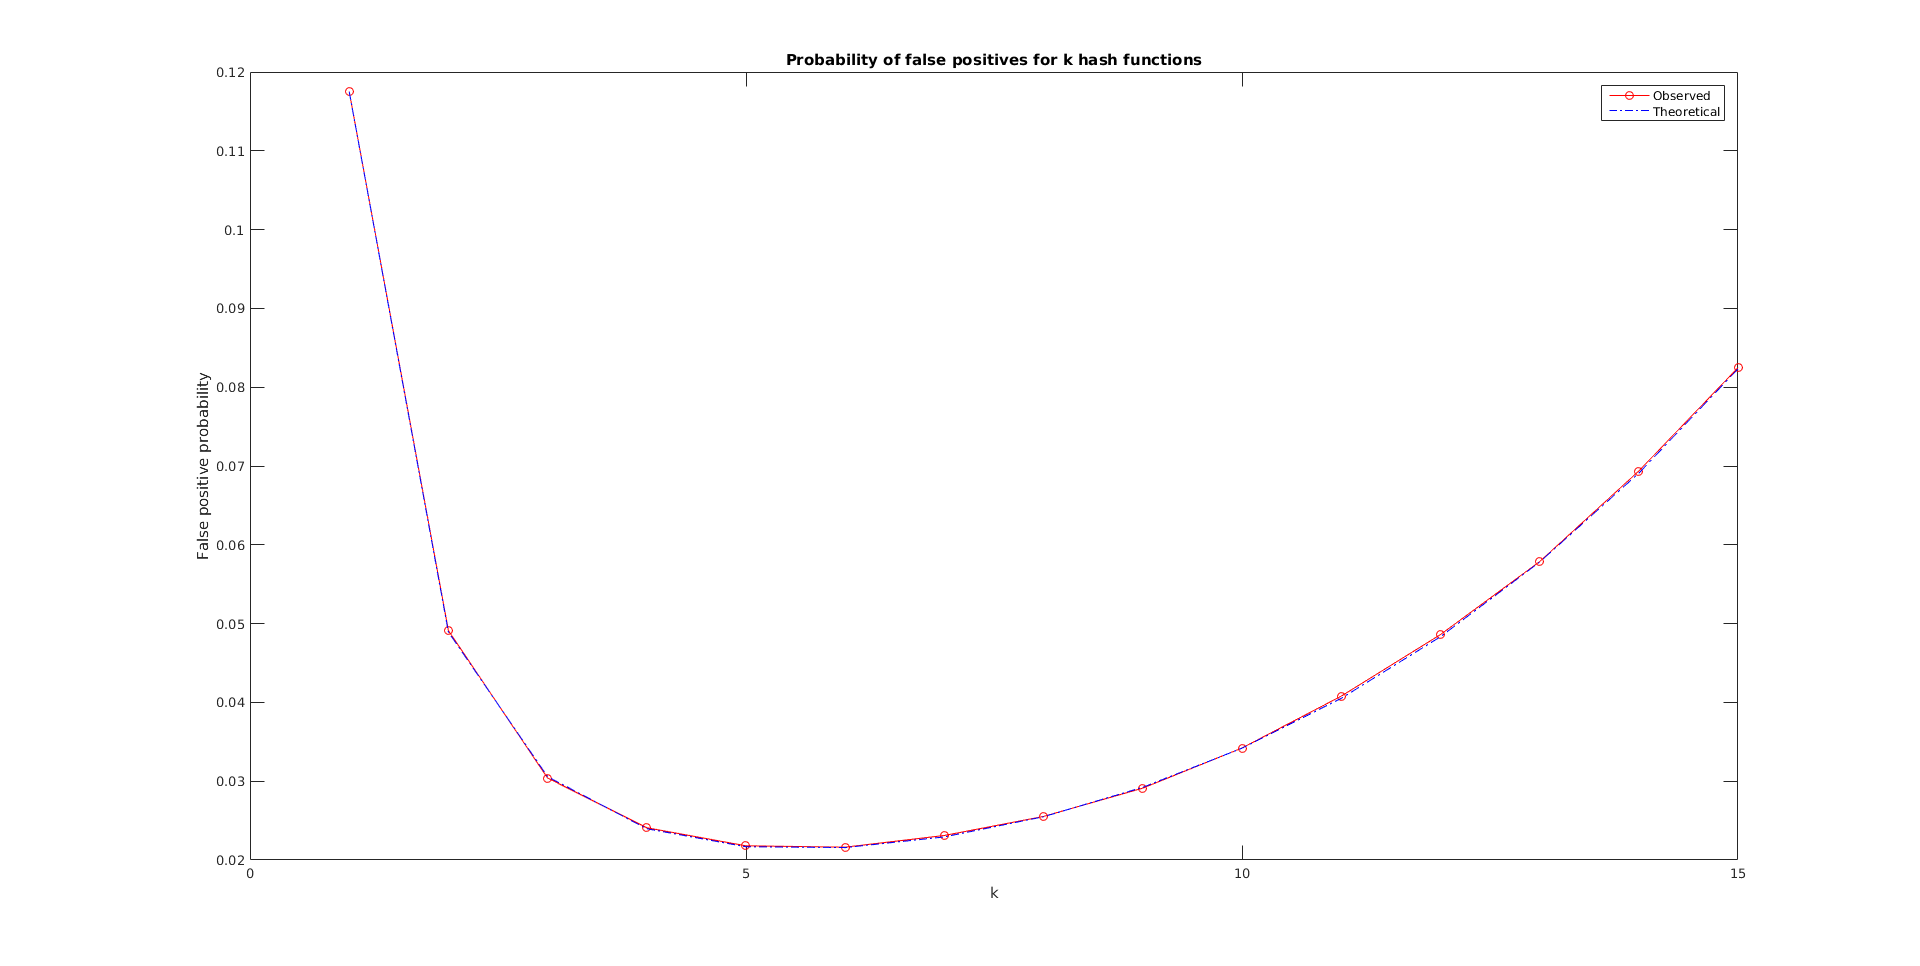
\includegraphics[height=5cm]{img/test_OptimalK}}
\caption{Resultados do teste do número ideal de funções de \textit{hashing} (\texttt{k})}
\label{fig:optimalk}
\end{figure}

\subsection{Tamanho ideal do vetor de \textit{bytes}}
\label{subsec.optimaln}

O módulo para o teste do valor ideal do tamanho \texttt{n} do vetor encontra-se no ficheiro \textit{test\_optimalN.m}.

Tal como no teste do \autoref{subsec.optimalk}, também são criados dois conjuntos de \textit{strings} aleatórias com o mesmo propósito, um para ser adicionado ao filtro e o outro não. É também criado um vetor com diferentes valores de \texttt{n}, que vão desde o tamanho do conjunto de \textit{strings} a adicionar até 10 vezes esse valor, com um incremento de metade do tamanho do conjunto entre cada.

De seguida, itera-se sobre os valores deste último vetor, criando-se uma instância de um \textit{Bloom-filter} com os valores de \texttt{n} (atributo \texttt{arraySize} do módulo) e \texttt{k} (que depende do tamanho do vetor) a cada passagem. Adiciona-se um dos conjuntos de \textit{strings}, verifica-se a existência dos elementos do outro que não foi adicionado e, por fim, calcula-se a probabilidade de falsos positivos, de maneira semelhante ao que foi feito no teste anterior. Vai sendo também calculado para cada valor de \texttt{n} o valor teórico correspondente da probabilidade de falsos positivos, e guardando estes valores num segundo vetor.

Como se verifica no gráfico da \autoref{fig:optimalnimg}, à medida que o tamanho do \textit{array} aumenta, a probabilidade de falsos positivos diminui, i.e., são inversamente proporcionais (o que está de acordo com o esperado). No entanto o mais importante com este teste é verificar que os valores experimentais são semelhantes aos teóricos, já que o importante será para um dado valor de erro admissível, dimensionar o \textit{array} interno eficientemente (pois caso contrário ou se vai ocupar memória desnecessária, ou o número de falsos positivos real será acima do admissível). Como os valores obtidos (experimentais e teóricos) são bastante semelhantes, conlui-se que a dedução teórica que é utilizada no construtor do filtro permite um bom dimensionamento da estrutura de dados interna deste.

\begin{figure}[ht]	
\center
\fbox{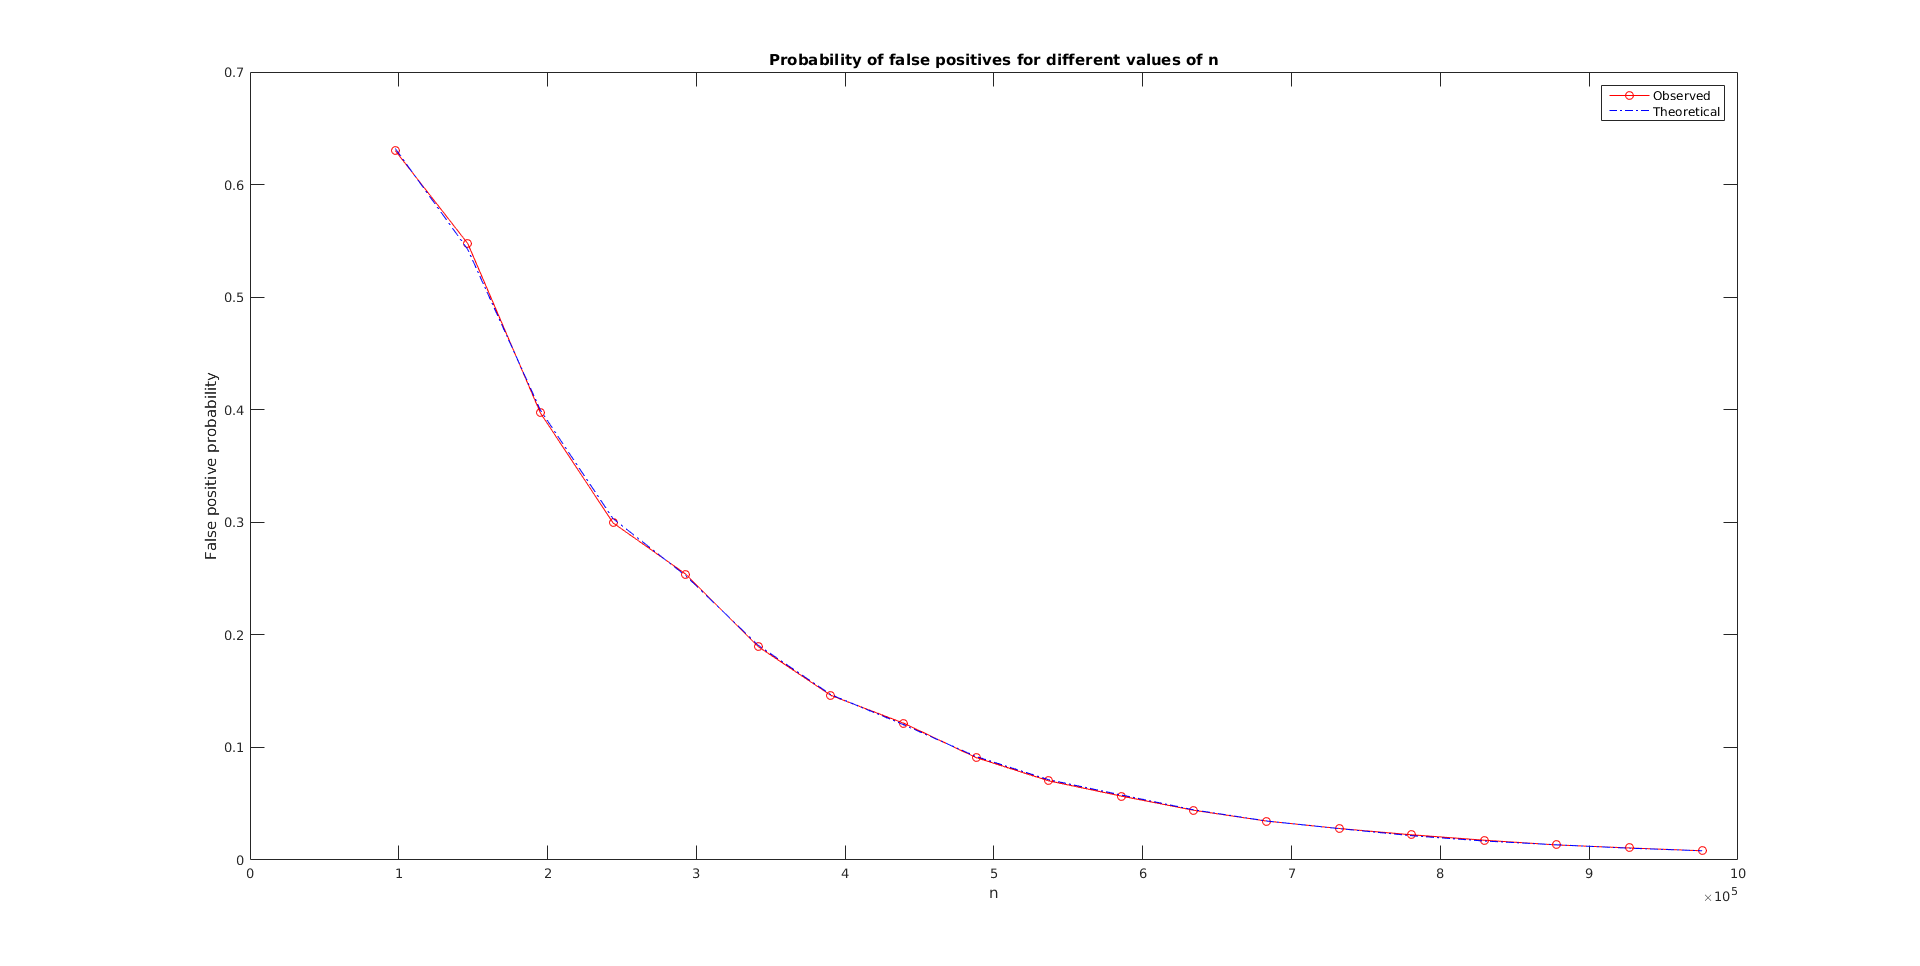
\includegraphics[height=5cm]{img/test_OptimalN_img}}
\caption{Resultados do teste do tamanho ideal do vetor de \textit{bytes} (\texttt{arraySize} ou \texttt{n})}
\label{fig:optimalnimg}
\end{figure}

Os valores ideias são os presentes na \autoref{fig:optimalntext}.

\begin{figure}[ht]	
\center
\fbox{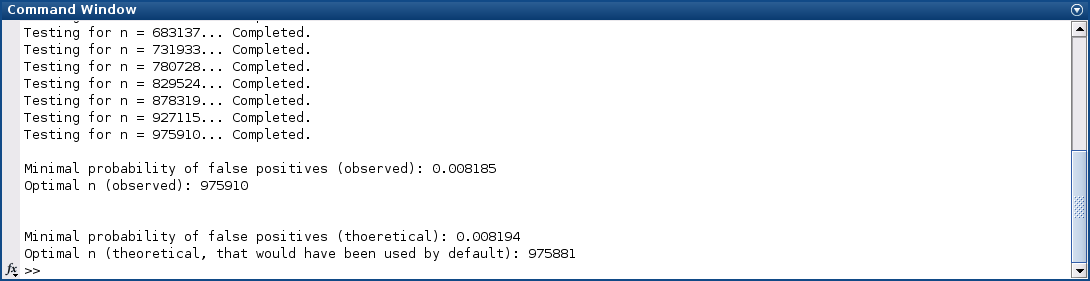
\includegraphics[height=5cm]{img/test_OptimalN_txt}}
\caption{Resultados ideias do tamanho ideal do vetor de \textit{bits} (\texttt{arraySize} ou \texttt{n})}
\label{fig:optimalntext}
\end{figure}

\subsection{Testes práticos do \textit{Bloom-filter}}
\label{subsec.testebloom}

Foram desenvolvidos dois módulos semelhantes para testeS mais direcionadoS ao uso real de um \textit{Bloom-filter}. Estão em dois ficheiros distintos, \textit{test\_big\_BloomFilter.m} e \textit{test\_small\_BloomFilter.m}.

O primeiro segue o modelo dos testes anteriores, em que se gera dois \textit{sets} de um certo tamanho (neste caso, cem mil elementos) de \textit{strings} aleatórias, cria-se uma instância de um \textit{Bloom-filter} com uma probabilidade de falsos positivos de 0.0001\%, adiciona-se um dos conjuntos ao filtro e verifica-se a ocurrência de falsos positivos com o outro. Por fim, compara-se o resultado observado da probabilidade de falsos positivos com a que se definiu aquando a criação do filtro. O objetivo é que os resultados sejam o mais próximos possíveis, o que se verificou em ambos os testes.

No segundo teste (\textit{small}), contrariamente ao primeiro em que se geram os conjuntos, definem-se conjuntos muito pequenos inicialmente e, depois, executa-se o mesmo processo que anteriormente.

\begin{figure}[ht]	
\center
\fbox{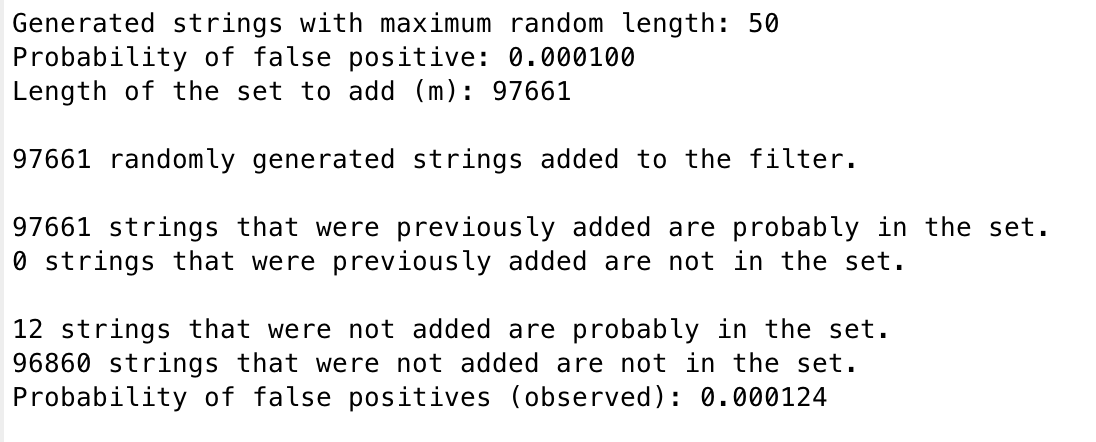
\includegraphics[height=5cm]{img/test_big_BloomFilter}}
\caption{Resultados da execução de \textit{test\_big\_BloomFilter.m}}
\label{fig:testbigbloom}
\end{figure}

\chapter{Locality-Sensitive Hashing}
\label{chap.lsh}

\textit{Locality-Sensitive Hashing (LSH)} é particularmente útil quando se têm por exemplo grandes conjuntos de documentos e se pretende encontrar aqueles semelhantes entre si, como, por exemplo, encontrar notícias semelhantes (em conteúdo) em diversos \textit{websites}. Muitas das vezes com conjuntos com tamanho na ordem dos milhões, são tantas as comparações necessárias a fazer e a memória necessária para guardar os documentos, que se torna inviável a utilização de métodos ``clássicos'', por exemplo comparando os documentos no seu todo um a um.

Com o objetivo de implementar um módulo capaz de efetuar a procura pelos vizinhos mais próximos (\textit{nearest neighbor search}), guardando representações de documentos mais facilmente comparáveis e que ocupam geralmente menos espaço, seguiram-se três passos:

\begin{description}
\item[Shingling]
Converter documentos para conjuntos de elementos (habitualmente pequenas \textit{strings}) denominados \textit{shingles}, o que permite uma melhor representação do conteúdo de um documento. Neste trabalho escolheu-se uma técnica de extração de \textit{shingles} sugerida em \cite{book1}, se procura por \textit{stopping words} e, para cada palavra encontrada, forma-se um \textit{shingle} constituído pela palavra e pelas duas palavras seguintes.
\item[Minhashing]
Converter grandes conjuntos (usualmente de \textit{shingles}) para uma pequena assinatura (por norma, vetor de \textit{hash codes}), preservando o conceito de similariedade entre diferentes documentos (neste caso, conjuntos de \textif{shingles}).
\item[Locality-sensitive hashing]
Reduzir o conjunto de elementos a candidatos de forma eficiênte, testando mais tarde a sua ``real'' similariedade.
\end{description}

O módulo de \textit{LSH} está escrito no ficheiro \textit{LSH.m} e dispõe dos seguintes métodos:

\begin{description}
\item[shingleWords]
Aceita um \textit{cell array} com as palavras (\textit{strings}) que constituem um documento e devolve um conjunto de \textit{shingles} relativos ao mesmo, construído tendo em conta um conjunto de \textit{stopping words}.
\item[signature]
Converte um conjunto (mais precisamente \textit{cell array}) de \textit{shingles} numa assinatura (vetor de inteiros), recorrendo a um processo de \textit{minhashing}.
\item[candidates]
Devolve a lista de documentos candidatos a formarem conjuntos semelhantes, consoante a matriz de assinaturas e o \textit{threshold} passados como argumentos.
\item[candidates\_to]
Executa um processo smelhante ao da função \texttt{candidates}, no entanto em vez de formar conjuntos de candidatos pra uma dada matriz de assinaturas, forma uma lista de candidatos (representados numa matriz de assinaturas), face a um documento específico (representado pela sua assinatura e passada como argumento).
\item[similars]
Verifica quais são os documentos de um conjunto de candidatos realmente semelhantes, consoante a matriz de candidatos, assinaturas e o \textit{threshold} passados como argumentos.
\item[similiars\_to]
Semelhante à função \texttt{similars}, no entanto aplica-se ao caso em que pretendemos comparar os candidatos a similares entre um único documento e outro conjunto de documentos (sendo os documentos tal como habitualmente representados pelas suas assinaturas).
\end{description}

O construtor do módulo aceita apenas um argumento (\texttt{expectedError}) que é o erro esperado quando se calcula a similaridade entre dois conjuntos representados pelas suas assinaturas obtidas segundo o método de \textit{Minhash}, face à real similaridade de Jaccard entre esses conjuntos. Este valor é utilizado para calcular o tamanho \texttt{k} das assinaturas (e portanto o número de funções de dispersão necessárias). (\texttt{k}) é o único atributo que o módulo possui (não considerando o atributo \texttt{debug} utilizado em \textit{debugging}), e é calculado utilizando a fórmula

$$ k = 1 / expectedError^2 $$

Este resultado é obtido pelos limites de Chernoff (\href{https://en.wikipedia.org/wiki/Chernoff\_bound}{Chernoff bounds}), concluindo-se que o erro esperado para o cálculo da similaridade de dois conjuntos segundo o método de \textit{Minhash} é $\mathcal{O}(\frac{1}{\sqrt{k}}$.

\subsection{Shingling}
\label{subsec.shingling}

Um \textit{k-shingle} de um documento é uma sequência de \textit{k tokens} (palavras, caracteres, etc.) que aparecem no documento. Documentos que tenham muitas \textit{shingles} em comum, possuem texto parecido, mesmo que este não apareça na mesma ordem. Este facto é importante pois permite determinar a semelhança entre diferentes documentos tendo em conta a ordem segundo a qual diferentes palavras aparecem (considere-se que facilmente se escrevem dois textos com paroximadamente as mesmas palavras mas em que, dada a ordem segundo a qual estas aparecem, o conteúdo destes documentos é bastante diferente).

A similariedade entre dois documentos ($D1, D2$) pode ser calculada através da similariedade de Jaccard:

$$ sim(D1, D2) = \frac{|C1\cap C2|}{|C1\cup C2|} $$

sendo $C1$ e $C2$ os conjuntos de \textit{shingles} de $D1$ e $D2$, respetivamente.

A distância de Jaccard, por outro lado, pode ser dada por:

$$ d(D1, D2) = 1 - sim(D1, D2) $$

Para gerar um \textit{set} de \textit{shingles} é utilizada a função \texttt{shingleWords} do módulo escrito, que recebe como argumento um \textit{cell array}, neste caso, de \textit{strings} que contém as palavras do documento (considere-se \texttt{Doc}) para o qual se quer gerar o conjunto de \textit{shingles}. Para gerar esse conjunto, é necessário selecionar quais as sequências de palavras mais importantes de \texttt{Doc}. Para tal e seguindo o algoritmo sugerido em \cite{book1}, é necessária a criação de um \textit{set} de \textit{stop words}. Estas palavras devem ser palavras que apareçam com grande frequência na língua considerada e que geralmente aparecem próximas de palavras importantes no contexto de um documento. Assim e para este efeito, foram guardadas num \textit{cell array} as cem palavras mais comuns da língua inglesa. Quando o programa encontra uma \textit{stopping word}, guarda a sequência \textit{stop\_word next\_word1 next\_word2} num segundo \textit{cell array}, que será o retorno da função.

\subsection{Minhashing}
\label{subsec.minhash}

Para contornar as demoras que as comparações de excertos de textos provocariam, os \textit{shingles} são convertidos em assinaturas de inteiros, no entanto, a similariedade entre documentos deve manifestar-se também nestas assinaturas.

Para sua criação é usada a função \texttt{signature}: começa-se por se criar um vetor com tamanho \texttt{k} tal como definido no construtor do módulo, em que os seus valores iniciais são o valor máximo do tipo \textit{unsigned integer 64-bits} (considerado como $+\infty$ no cálculo dos valores mínimos) e, de seguida, para cada valor \textit{seed} inicialmente igual a $1$ e variando até \texttt{k} (número de \textit{hash functions}), é gerado um vetor das \textit{hash codes} para o \textit{cell array} de \textit{shingles} passado como argumento, e para esse valor de \textit{seed}. É depois calculado o mínimo desse vetor, guardando-se o resultado na posição \textit{seed} do vetor assinatura que será no final devolvido pela função.

\subsection{Locality-sensitive hashing}
\label{subsec.lsh}

Por fim, depois de geradosgeradas as assinaturas dos documentos, estas podem ser comparadas para se determinar os documentos que mais se assemelham.

Para isso inicialmente começa-se por se definir uma lista de candidatos possíveis (onde é ``provável'' a ocorrência de falsos positivos), para, mais tarde, se verificar quais aqueles que são realmente semelhantes. É por isso necessário definir um valor de \textit{threshold} que deverá indicar quão semelhantes dois documentos devem ser para poderem ser considerados similares, no contexto do problema considerado.

A função \texttt{candidates} definida no módulo \texttt{LSH} serve para calcular a lista de candidatos possíveis. Consideremos a matriz de assinaturas \textit{S}, onde cada coluna corresponde à assinatura de um documento (i.e., o resultado do processo de \textit{Minhhashing} dos \textit{shingles} obtidos).

Esta matriz é dividida em \texttt{b} bandas (\textir{bands}) de \texttt{r} linhas (\textit{rows}) cada. Então, para cada banda verificam-se quais as colunas (da banda) iguais - estes elementos serão considerados candidatos e serão portanto adicionados ao \textit{cell array} de candidados que será devolvido.

Tendo em conta que

$$ br = k,\ k\ \text{tamanho de cada assinatura} $$

e

$$ t \approx \left(\frac{1}{b}\right) ^ {\frac{1}{r}} $$

onde $t$ é o \textit{threshold} escolhido, pode aproximar-se \texttt{b} ou \texttt{r} e em função do valor calculado, obter o outro.

A estrutura da matriz de retorno (\textit{cell array} de candidatos) é tal que cada linha \textit{i} corresponde ao documento \textit{i} e cada elemento dessa linha corresponde ao documento \textit{j}, significando que esse par \textit{(Docs{i}, Docs{j})} constitui um par de candidatos (i.e., o documento \textit{i} poderá ser semelhante ao documento \textit{j}).

No final da execução da função deverá obter-se um \textit{cell array} com todos os pares de candidatos a serem semelhantes. É de notar que na abordagem seguida tenta-se eliminar entradas irrelevantes, ou seja, se a matriz de candidatos indica que poderá haver semelhança entre \textit{Docs{i}} e \textit{Docs{j}}, então não deverá indicar o equivalente \textit{Docs{j}} ``semelhante a'' \textit{Docs{i}}.

Por fim, a função \texttt{similars} trata de finalizar o processo e devolver os pares de documentos que são realmente semelhantes, incluindo o respetivo coeficiente de similariedade.

Para isso itera-se sobre a matriz de candidatos e compara-se, um a um, se a similariedade de Jaccard entre as assinaturas é maior ou igual ao \textit{threshold} definido (usando a função \texttt{intersect}, que devolve os elementos em comum entre dois conjuntos). Se a condição se verificar, adiciona-se ao vetor de retorno os índices na matriz de assinaturas dos documentos em questão e o valor da sua similariedade.

\subsection{Testes}
\label{subsec.lshtests}

Para os testes deste módulo, foram adaptados os \textit{scripts} do Guião Prático-Laboratorial 07 da disciplina, mas, para além de ser usado o \textit{dataset} de cem mil utilizadores da MovieLens, foi também utilizado o que contém um milhão de utilizadores.

A única diferença entre os testes é apenas o \textit{dataset} utilizado, pois o processo tem obrigatoriamente de ser o mesmo, apenas variando o tamanho do conjunto de dados.

Inicia-se o teste obtendo um vetor com todos os utilizadores a partir do \textit{dataset}. De seguida, para cada utilizador, constrói-se o conjunto de \textit{shingles} (neste caso, não é usada a função \texttt{shingleWords} do módulo \texttt{LSH}, visto que não é um documento de texto, mas sim o vetor de índices de filmes, que são convertidos para \textit{strings} para poderem ser utilizados diretamente, que cada utilizador avaliou) e respetivas assinaturas, usando a função \texttt{signature}. 

Primeiro é calculada a similariedade de Jaccard esperada (teórica), simplesmente iterando sobre o conjunto de assinaturas e utilizando a expressão 

$$ sim(D1, D2) = \frac{|C1\cap C2|}{|C1\cup C2|} $$

e as funções de MATLAB \textit{intersec} (devolve os elementos que dois conjuntos têm em comum) e \texttt{union} (devolve a união de dois conjuntos) (é ainda utilizada a função \textit{length} pois apenas importa o tamanho dos conjuntos que as duas funções anteriores devolvem). Por fim, verifica-se, quais destes valores estão acima do \textit{threshold} assumido (nestes teste, assumiu-se 0.6). Os resultados mostram que existem apenas 3 documentos com similariedade acima dos 0.6, como se verifica na \autoref{fig:test100ke}.

\begin{figure}[ht]	
\center
\fbox{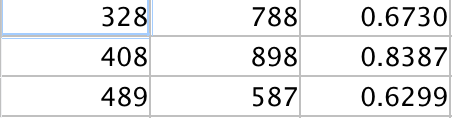
\includegraphics[height=2cm]{img/test_LSH_100k_Exp}}
\caption{Resultados (valores esperados) do teste com 100 mil utilizadores}
\label{fig:test100ke}
\end{figure}

Finalmente, para calcular a similariedade de Jaccard observada (experimental), gera-se a lista de candidatos usando a função \texttt{candidates} do módulo \texttt{LSH} e a matriz com os documentos similares usando a função \texttt{similars}, também do mesmo módulo.

A \autoref{fig:test100ko} mostra que os resultados de ambos os testes foram os mesmos, havendo apenas uma pequena variação dos valores de similariedade (à volta de 0.02). Note-se que a instancia de \textit{LSH} utilizada foi inicializada para um erro de 0.05, e portanto como $0.02 < 0.05$ os resultados estão de acordo com o esperado.

\begin{figure}[ht]
\center
\fbox{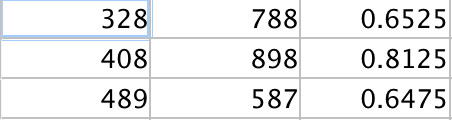
\includegraphics[height=2cm]{img/test_LSH_100k_Obs}}
\caption{Resultados (valores observados) do teste com 100 mil utilizadores}
\label{fig:test100ko}
\end{figure}

% Falta teste com dataset de 1m

\chapter{SPAM Filter}
\label{chap.spamfilter}

A filtragem de \textit{email} é uma maneira de o organizar segundo um dado critério, por exemplo detetar \textit{spam} evitando assim ter de ler mensagens sem interesse. Neste trabalho considera-se \textit{spam} como sendo mensagens que para um dado utilizador não têm interesse (ou seja, o que é \textit{spam} para uma pessoa poderá não o ser para outra), e portanto poderá ser visto como apenas mais uma forma de categorizar \textit{emails}.

Uma maneira de filtrar o \textit{spam} de uma caixa de entrada é comparar o conteúdo de \textit{emails} previamente consideramos como tal e ver se são semelhantes à mensagem que se acabou de receber - se sim, colocar a mensagem na pasta certa, se não então nada fazer. Outro método é verificar se o endereço de \textit{email} da nova mensagem já enviara algum \textit{email} de \textit{spam} anteriormente.

Estas funcionalidades são geralmente oferecidas por empresas como a Google ou Microsoft, que habitualmente utilizam algoritmos que detetam por exemplo picos de atividade de determinados endereços (especialmente se até então desconhecidos), bem como \textit{feedback} dos seus utilizadores que marcam ou não como \textit{spam} os \textit{emails} que recebem. A par disto, muitas vezes as mensagens que levantam mais dúvidas são são verificados por equipas com essa tarefa.

Neste trabalho pretende-se implementar um simples filtro de \textit{spam} (ou qualquer outro tipo de mensagens), utilizando para isso um \textit{Bloom-filter} (de forma a filtrar facilmente por endereço) e técnicas de \textit{Locality-sensitive hashing} (para se filtrar por conteúdo), já que estes deverão ser particularmente úteis nestas matérias.

O \textit{Bloom-filter} servirá como armazenamento de endereços de \textit{email} que previamente tinham enviado lixo, constituindo assim uma \textit{backlist} de mensagens que deverão ser imediatamente filtradas. Já \textit{Locality-sensitive hashing} servirá para comparar o conteúdo de novas mensagens com antigas mensagens marcadas como \textit{spam}, permitindo assim inferir novas mensagens como sendo de interesse ou não. Algumas das principais vantagens desta abordagem são a facilidade com que pode ser implementada, bem como a eficiência de filtragem que pode permitir não só em termos de velocidade de execução mas também permitindo por exemplo que cada utilizador tenha facilmente a sua própria lista de \textit{emails} sem interesse.

Os passos necessários para a filtragem segundo este modelo serão:

\begin{description}
\item[Aprendizagem] \hfill \\
  Esta fase deverá ser executada uma vez. Aqui o programa deve aprender a que se assemelha \textit{spam}, permitindo mais tarde filtrar mensagens semelhantes. Para isso deverão ser fornecidos ao programa \textit{emails} considerados como \textit{spam}, e o programa em troca deve não só armazenar os remetentes destas mensagens num \textit{Bloom-filter} para referência futura, como também gerar e guardar uma assinatura segundo a técnica de \textit{Minhash} para o corpo da mensagem. Este último passo é executado conforme indicado anteriormente no que toca à criação de um conjunto de \textit{shingles} para um documento, bem como à posterior geração da assinatura desse conjunto. Estas assinaturas vão sendo guardadas numa matriz onde cada coluna é referente à assinatura de um \textit{email} de \textit{spam}.
\item[Verificação 1] \hfill \\
  Neste momento o modelo utilizado já conhece o que é \textit{spam}, e portanto está apto a filtrar este tipo de mensagens. Nesta primeira fase de filtragem, deverá ser verificado se o endereço do remetente é ou não um endereço \textit{blacklisted}. Note-se que visto que o \textit{Bloom-filter} deste trabalho foi implementado como um \textit{Counting filter}, poderá ser mais proveitoso não apenas verificar se um endereço pertence ou não ao filtro, mas antes verificar se a contagem para esse endereço é superior a um determinado valor.
\item[Verificação 2] \hfill \\
  Caso a mensagem passe na verificação acima, então passa-se a uma fase onde o conteúdo da mensagem é analisado contra o conhecimento que o modelo tem do que é \textit{spam}. Também esta verificação é dividida em vários passos:
  \begin{enumerate}
  \item Começa-se por se gerar o conjunto de \textit{shingles} referente ao \textit{email}. Caso este forme um conjunto vazio, então imediatamente conclui-se que a mensagem é \textit{spam} já que nenhuma informação relevante foi obtida. Caso contrário, calcula-se a assinatura do \textit{email} e avança-se para a fase seguinte. \\
    A construção do conjunto de \textit{shingles} e da assinatura do \textit{email} é conforme o já referido anteriormente.
  \item Conhecendo a assinatura da mensagem e possuindo a matrz de assinaturas de \textit{emails} de \textit{spam}, calcula-se a lista de candidatos da matriz de assinaturas a serem semelhantes à assinatura da mensagem a avaliar atualmente. Isto é possível recorrendo ao método \texttt{candidates\_to} do módulo \textit{LSH}, que funciona tal como a função homóloga \texttt{candidates}, com a diferença de que a primeira calcula os candidatos face a um determinado documento (e não todos os conjuntos de candidatos possíveis como a segunda). \\
    Caso seja retornada um conjunto vazio, então conclui-se que a mensagem atual não se assemelha a \textit{spam} e portanto a verificação termina indicando que a mensagem é com interesse. Caso contrário, avança-se para a fase seguite.
  \item Por fim, a partir da lista de candidatos gerada na fase anterior calculam-se as verdadeiras semelhanças entre as diferentes assinaturas dos candidatos, a partir da função \texttt{similars\_to} que faz as vezes da função \texttt{similars}, com a diferença de que a primeira é também específica para calcular assinaturas similares a um só assinatura, ou contrário da segunda que calcula os pares similares para todos os elementos da matriz de candidatos. Caso seja devolvida uma matriz vazia, o passo anterior apenas devolveu falsos positivos e portanto a mensagem não é considerada \textit{spam}, caso contrário o conteúdo da mensagem assemelhou-se a algum outro doutra mensagem que tinha sido aprendida (como \textit{spam}), e portanto conluí-se que esta deve também ser uma mensagem sem interesse.
  \end{enumerate}
\end{description}

Note-se que nos dois pontos da descrição anterior, as duas funções utilizadas utilizam um valor de \textit{threshold}, passado como argumento, que deve ser definido tendo em conta dois fatores: um valor muito elevado, garantirá que muito poucas mensagens que não são \textit{spam} sejam detetadas como tal, por outro lado poderá estar-se a não filtrar mais mensagens que são efetivamente \textit{spam}. O contrário acontece para valores muito baixos de \textit{threshold}, onde quase todos os \textit{emails} de \textit{spam} serão filtrados, mas também mais mensagens com interesse podem ser filtradas.

Assim, primeiro é necessário que o programa ``aprenda'' que \texit{emails} deve filtrar. Para tal, em dois testes foram utilizado dois \textit{datasets} diferentes, um do grupo \textit{CSMining}\footnote{\url{http://csmining.org/index.php/spam-email-datasets-.html}}, outro do grupo \textit{Enron}\footnote{\url{http://csmining.org/index.php/enron-spam-datasets.html}}. A função \texttt{create\_generic} permite a aprendizagem, aceitando um diretório onde vai procurar pelos ficheiros da extensão que também lhe é passada como argumento, para guardar num ficheiro (o caminho também é passado como argumento) as estruturas \textit{Bloom-filter} com os endereços de \textit{email} que enviaram \textit{spam} adicionados, as assinaturas do conteúdo dos mesmos e o módulo de \textit{LSH} usado (para salvaguardar o número de funções de \textit{hashing} utilizadas).

Por outro lado, a função \texttt{test\_generic} testa o filtro de \textit{spam} com base no ficheiro previamente guardado. Os dados desse mesmo ficheiro são carregados para o programa e todos os \textit{emails} contidos na pasta que lhe é passada como argumento são analisados.

É de notar que o método descrito acima para filtragem de \textit{spam} pode ser facilmente utilizado para filtrar por tema, permitindo por exemplo categorizar \textit{emails} com três \textit{labels}, \textit{Primary}, \textit{Social} e \textit{Promotions} à semelhança do que o \textit{Gmail} da Google faz. Basta para isso fornecer um conjunto de aprendizagem adequado. O programa pode também aprender com a experiência a melhorar os seus resultados, bastando para isso que, quando falha a filtragem de uma mensagem e o utilizador o assinale, seja adicionado o endereço do remetente ao filtro de \textit{Bloom} em uso e a assinatura da mensagem à matriz de assianturas que já possui.

\section{Testes}

Os testes levados a cabo nesta fase foram os menos claros de todo o projeto, dada a falta de dados para testar eficientemente o programa...

\section{Programa \textit{demo}}

Foi desenvolvido ainda um programa \textit{demo} (\textit{proof\_of\_concept.m})  que pretende funcionar como \textit{proof of concept} do modelo. Para isso, foram testados \textit{emails} que recorrentemente são recebidos pelos autores deste projeto. Com um \textit{use case} específico pretende-se mostrar como funciona efetivamente o programa.

Assim, começou-se por se juntar um conjunto de cerca de 40 \textit{emails} que são por nós considerados como lixo (no entanto poderão ser mensagens com interesse para outras pessoas e portanto não são filtradas por definição por serviços de \textit{email} como o \textit{Gmail}). Guardou-se depois um pequeno número de \textit{emails} que são consideradas com interesse e verificou-se se alguma destas mensagens era filtrada como \textit{spam} pelo programa. Posto isto e para efeitos demonstrativos, o programa entra num \textit{loop} onde permite a verificação de outras mensagens sem que estas tenham de ser previamente preprocessadas. O resultado é o ilustrado na \autoref{fig:poc1}.

\begin{figure}[ht]	
\center
\fbox{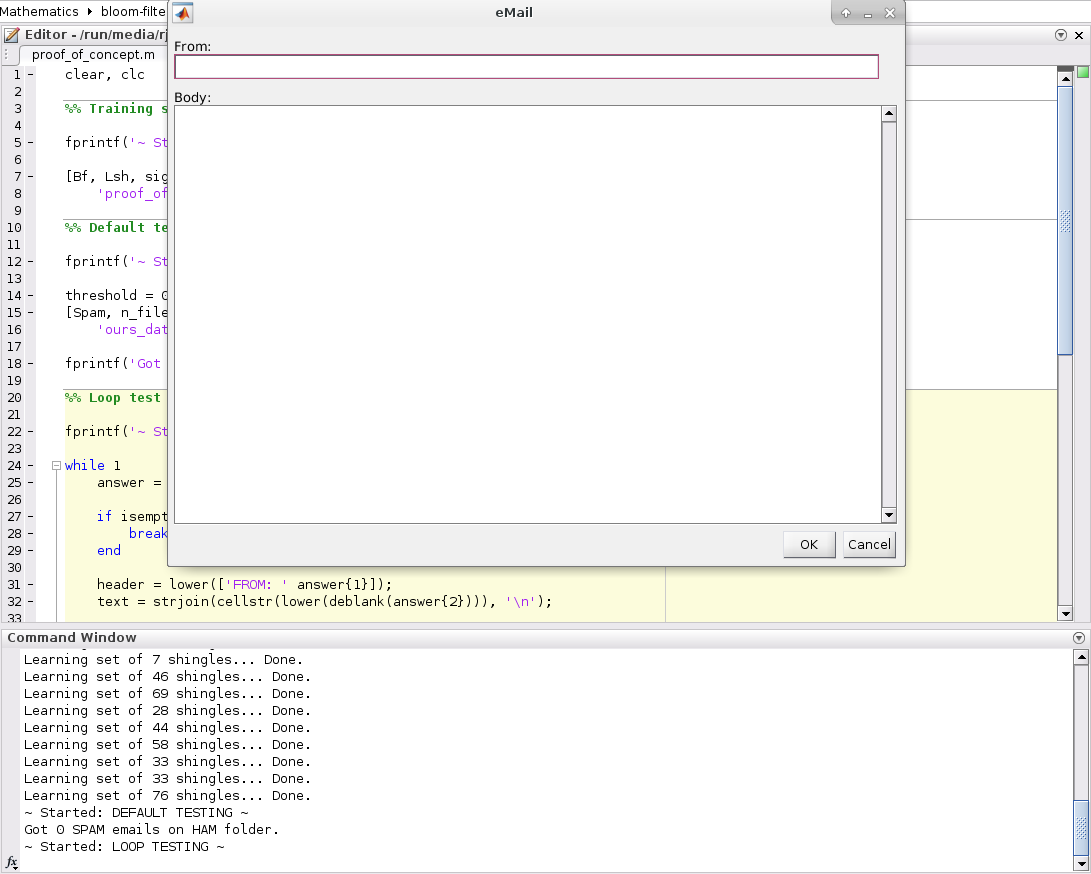
\includegraphics[height=2cm]{img/proof_of_concept1}}
\caption{Resultados da execução do programa \textit{demo} + janela para teste de novos \textit{emails}}
\label{fig:poc1}
\end{figure}

Neste teste conseguiu-se filtrar as mensagens sem interesse, ao mesmo tempo que as relevantes não eram afetadas.

\chapter{Conclusões}
\label{chap.conclusões}

\maketitle
\nocite{*}
\printbibliography[title={Referências}]

\end{document}
